\documentclass[border=3pt,tikz]{standalone}
\usepackage{amsmath} % for aligned
\usetikzlibrary{arrows.meta} % for arrow size
\usetikzlibrary{fit, positioning, backgrounds, scopes} % For labels, boxes, scopes
\usepackage[outline]{contour} % glow around text
\contourlength{1.4pt}

% COLORS
\usepackage{xcolor}
\colorlet{myred}{red!80!black}
\colorlet{myblue}{blue!80!black}
\colorlet{mygreen}{green!60!black}
\colorlet{myorange}{orange!70!red!60!black}
\colorlet{mydarkred}{red!30!black}
\colorlet{mydarkblue}{blue!40!black}
\colorlet{mydarkgreen}{green!30!black}

% STYLES
\tikzset{
  >=latex, % for default LaTeX arrow head
  node/.style={thick,circle,draw=myblue,minimum size=20,inner sep=0.5,outer sep=0.6},
  node in/.style={node,green!20!black,draw=mygreen!30!black,fill=mygreen!25},
  node trunk/.style={node,blue!20!black,draw=myblue!30!black,fill=myblue!20},
  node head/.style={node,orange!20!black,draw=myorange!30!black,fill=myorange!20},
  node out/.style={node,red!20!black,draw=myred!30!black,fill=myred!20},
  connect/.style={thick,mydarkblue},
  label/.style={font=\small,align=center},
  box/.style={draw, thick, rounded corners, inner sep=10pt, fill opacity=0.05}
}

\begin{document}

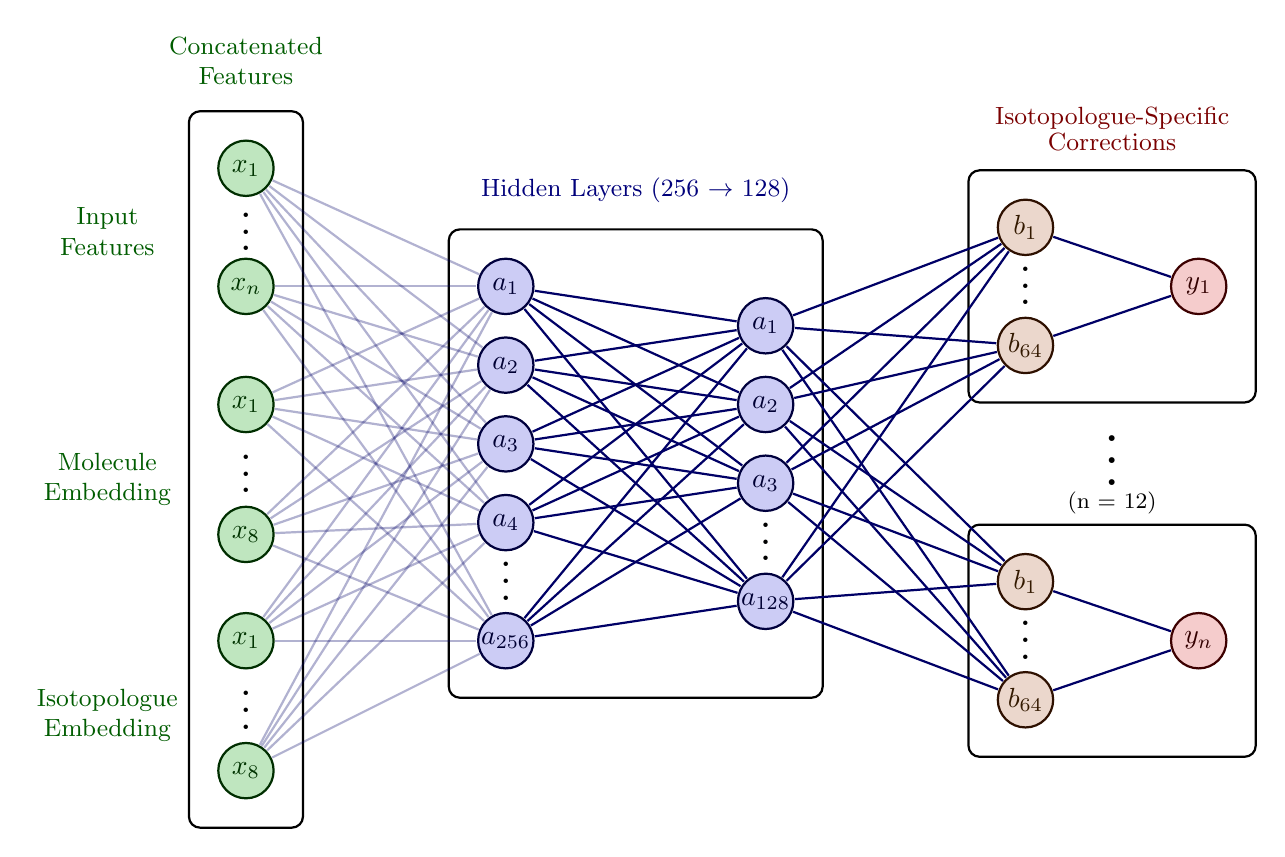
\begin{tikzpicture}[x=2.2cm,y=1.0cm]
  
  % --- LAYER 1: INPUTS (x=1) ---
  % Group 1: Input Features (2 nodes)
  \node[node in] (N1-1) at (1, 5) {$x_1$};
  \node[node in] (N1-2) at (1, 3.5) {$x_n$};
  \path (N1-1) -- (N1-2) node[pos=0.5, yshift=0.1cm, scale=1.5] (dots-features) {$\vdots$};
  
  % Group 2: Molecule Embedding (2 nodes)
  \node[node in] (N1-m1) at (1, 2) {$x_1$};
  \node[node in] (N1-m2) at (1, 0.35) {$x_8$};
  \path (N1-m1) -- (N1-m2) node[pos=0.5, yshift=0.1cm, scale=1.5] (dots-mol) {$\vdots$};
  
  % Group 3: Isotopologue Embedding (2 nodes)
  \node[node in] (N1-i1) at (1, -1) {$x_1$};
  \node[node in] (N1-i2) at (1, -2.65) {$x_8$};
  \path (N1-i1) -- (N1-i2) node[pos=0.5, yshift=0.1cm, scale=1.5] (dots-iso) {$\vdots$};
  
  % Background box for inputs
  \begin{pgfonlayer}{background}
    \node[box, fit=(N1-1) (N1-i2), fill=mygreen!3] (input-box) {};
  \end{pgfonlayer}

  % Labels for input groups
  \node[label, mygreen!60!black, align=center] at (0.2, 4.2) {Input\\Features};
  \node[label, mygreen!60!black, align=center] at (0.2, 1.05) {Molecule\\Embedding};
  \node[label, mygreen!60!black, align=center] at (0.2, -1.95) {Isotopologue\\Embedding};

  % Label above input box
  \node[label, mygreen!60!black, align=center, above=2mm of input-box.north] {Concatenated\\Features};
  
  % --- LAYER 2: HIDDEN LAYERS (TRUNK) ---
  % --- TRUNK 1 (x=2.5) --- (256 nodes, 5 circles)
  \node[node trunk] (N2-1) at (2.5, 3.5) {$a_1$};
  \node[node trunk] (N2-2) at (2.5, 2.5) {$a_2$};
  \node[node trunk] (N2-3) at (2.5, 1.5) {$a_3$};
  \node[node trunk] (N2-4) at (2.5, 0.5) {$a_4$};
  \path (N2-4) -- ++(0,-1) node[pos=0.5, yshift=0.1cm, scale=1.5] {$\vdots$};
  \node[node trunk] (N2-5) at (2.5, -1) {$a_{256}$};
  
  % --- TRUNK 2 (x=4) --- (128 nodes, 4 circles)
  \node[node trunk] (N3-1) at (4, 3) {$a_1$};
  \node[node trunk] (N3-2) at (4, 2) {$a_2$};
  \node[node trunk] (N3-3) at (4, 1) {$a_3$};
  \path (N3-3) -- ++(0,-1) node[pos=0.5, yshift=0.1cm, scale=1.5] {$\vdots$};
  \node[node trunk] (N3-4) at (4, -0.5) {$a_{128}$};
  
  % --- CONNECTIONS: INPUT -> TRUNK 1 -> TRUNK 2 ---
  \foreach \i in {N1-1,N1-2,N1-m1,N1-m2,N1-i1,N1-i2} {
    \foreach \j in {1,2,3,4,5}{
      \draw[connect, opacity=0.3] (\i) -- (N2-\j);
    }
  }
  \foreach \i in {1,2,3,4,5} {
    \foreach \j in {1,2,3,4}{
      \draw[connect] (N2-\i) -- (N3-\j);
    }
  }
  
  % --- BACKGROUND BOX for TRUNK ---
  \begin{pgfonlayer}{background}
    \node[box, fit=(N2-1) (N2-5) (N3-1) (N3-4), fill=myblue!3] (trunk-box) {};
  \end{pgfonlayer}
  
  % Label above trunk box
  \node[label, myblue!60!black, align=center, above=2mm of trunk-box.north] {Hidden Layers (256 $\to$ 128)};
  
  % --- LAYER 3: ADAPTER HEADS ---
  % --- Head 1 (y-shifted up) ---
  \begin{scope}[yshift=3.25cm]
    % Head 1, Layer 1 (64 nodes, 2 circles with dots in middle)
    \node[node head] (N4-h1-1) at (5.5, 1) {$b_1$};
    \path (N4-h1-1) -- ++(0,-1) node[pos=0.5, yshift=0.1cm, scale=1.5] {$\vdots$};
    \node[node head] (N4-h1-2) at (5.5, -0.5) {$b_{64}$};
    
    % Head 1, Output (1 node)
    \node[node out] (N5-h1) at (6.5, 0.25) {$y_1$};
    
    % Connections from trunk to head
    \foreach \i in {1,2,3,4} {
      \foreach \j in {1,2}{
        \draw[connect] (N3-\i) -- (N4-h1-\j);
      }
    }
    \foreach \i in {1,2} {
      \draw[connect] (N4-h1-\i) -- (N5-h1);
    }
    
    % Box for head 1
    \begin{pgfonlayer}{background}
      \node[box, fit=(N4-h1-1) (N5-h1) (N4-h1-2), fill=myorange!3] (head1-box) {};
    \end{pgfonlayer}
    
    \end{scope}
  
  % --- Dots between heads (centered) ---
  \node[scale=2.0] at (6, 1.5) {$\vdots$};
  \node[label, align=center, font=\footnotesize] at (6, 0.75) {(n = 12)};
  
  % --- Head 2 (y-shifted down) ---
  \begin{scope}[yshift=-1.25cm]
    % Head 2, Layer 1 (64 nodes, 2 circles with dots in middle)
    \node[node head] (N4-h2-1) at (5.5, 1) {$b_1$};
    \path (N4-h2-1) -- ++(0,-1) node[pos=0.5, yshift=0.1cm, scale=1.5] {$\vdots$};
    \node[node head] (N4-h2-2) at (5.5, -0.5) {$b_{64}$};
    
    % Head 2, Output (1 node)
    \node[node out] (N5-h2) at (6.5, 0.25) {$y_n$};
    
    % Connections
    \foreach \i in {1,2,3,4} {
      \foreach \j in {1,2}{
        \draw[connect] (N3-\i) -- (N4-h2-\j);
      }
    }
    \foreach \i in {1,2} {
      \draw[connect] (N4-h2-\i) -- (N5-h2);
    }
    
    % Box for head 2
    \begin{pgfonlayer}{background}
      \node[box, fit=(N4-h2-1) (N5-h2) (N4-h2-2), fill=myorange!3] (head2-box) {};
    \end{pgfonlayer}
    
    \end{scope}
  
  % --- Output Label (centered above output heads, outside boxes) ---
  \node[label, myred!60!black, align=center] at (6, 5.5) {Isotopologue-Specific\\[-0.2em]Corrections};
  
\end{tikzpicture}

\end{document}